% A basic LaTeX document for an assignment

% If you want the title to appear on a separate
% page, change notitlepage to titlepage
\documentclass[11pt,a4paper,notitlepage]{article}
\usepackage[utf8]{inputenc}
\usepackage[T1]{fontenc}
% If your hand-in is in icelandic change english to icelandic
% Note: This has nothing to do with Icelandic characters, they
% can always be used. This just tells other packages what 
% language you are using and changes the hyphenation used by LaTeX
% If icelandic is selected, a shorthand, "` and "', is also included
% for Icelandic quotation marks. They can also obtained by using 
% ,, and ``
\usepackage[english]{babel}
\usepackage{amsmath, amsthm, amssymb, amsfonts}
\usepackage{graphicx}
\usepackage{enumerate}
% To use the whole A4-page
% See: ftp://ftp.tex.ac.uk/tex-archive/macros/latex/contrib/geometry/geometry.pdf
% and http://en.wikibooks.org/wiki/LaTeX/Document_Structure
\usepackage{geometry}
% For header and footer
% See: ftp://ctan.tug.org/tex-archive/macros/latex/contrib/fancyhdr/fancyhdr.pdf
% and http://en.wikibooks.org/wiki/LaTeX/Document_Structure
\usepackage{fancyhdr}
% For prettier tables
% See: http://ctan.mackichan.com/macros/latex/contrib/booktabs/booktabs.pdf
% and  http://en.wikibooks.org/wiki/LaTeX/Tables
\usepackage{booktabs}


%%%%%%%%%%%%%%%%%%%%%%%%%%% SETUP %%%%%%%%%%%%%%%%%%%%%%%%%%%

% Set the margins of the paper. By default LaTeX uses huge margins
\geometry{includeheadfoot, margin=2.5cm}
% you can also use
% \geometry{a4paper}
% End of margins setup

% Setup header and footer
% Headers
\pagestyle{fancy} % To get the header and footer
\lhead{\small \textsc{Lab Exercises}}
\rhead{\small \textsc{Introduction to Electronic Engineering}}
% Footers
%\lfoot{Left footer text}
%\cfoot{\thepage} % This is the default behaviour
%\rfoot{Right footer text}

% If you don't want a line below the header or above the footer, 
% change the appropriate header/footerrulewidth to 0pt
\setlength{\headheight}{15.2pt} % This is set to avoid a warning
\renewcommand{\headrulewidth}{0.4pt}
\renewcommand{\footrulewidth}{0.4pt}
% End of header and footer setup

% Setup Problem/Solution environments
\theoremstyle{plain}
\newtheorem{problem}{Problem}[section]

\theoremstyle{remark}
\newtheorem*{solution}{Solution}
% End of Problem/Solution environments setup

%%%%%%%%%%%%%%%%%%%%%%%% END OF SETUP %%%%%%%%%%%%%%%%%%%%%%%%

\title{{\large \bf \MakeUppercase{Introduction to Electronic Engineering}} \\
		\large \textsc{Lab exercises}}

\author{\textsc{\small Antal János Monori \& Emil Már Einarsson }}

\begin{document}
	\maketitle
	\large \bf{\textsc{\section{Lab 1}}
	\begin{problem}
		Problem 1 here.
	\end{problem}

	\begin{solution}
		Solution goes here.
	\end{solution}
	
	\begin{problem}
		Problem 1 here.
	\end{problem}
	
	\begin{solution}
		Solution goes here.
	\end{solution}
	
	\pagebreak

	\large \bf{\textsc{\section{Lab 2}}
	\begin{problem}
		Problem 1 here.
	\end{problem}
	
	\begin{solution}
		Solution goes here.
	\end{solution}
	
	\begin{problem}
		Problem 1 here.
	\end{problem}
	
	\begin{solution}
		Solution goes here.
	\end{solution}
	
	\pagebreak
	
	\large \bf{\textsc{\section{Lab 3}}
	\begin{problem}
		Choose a diode type 1N4001 and build the following circuit.\\	
		R=100 \(\Omega\) (potentiometer) \\ 
		D is 1N4001 \\
		E=2v (max current I$_{max}$=350mA)
		\newline\newline
		1. Measure the diode and resistor voltage and current when changing the resistor R and fill the table
		\newline
		2. Plot the I-V characteristics  of the diode as well as the resistor. Are all measurements on one line? Are the components linear? Compare the diode i-v plot with the datasheet.
		
		\begin{figure}[h!]
			\centering
			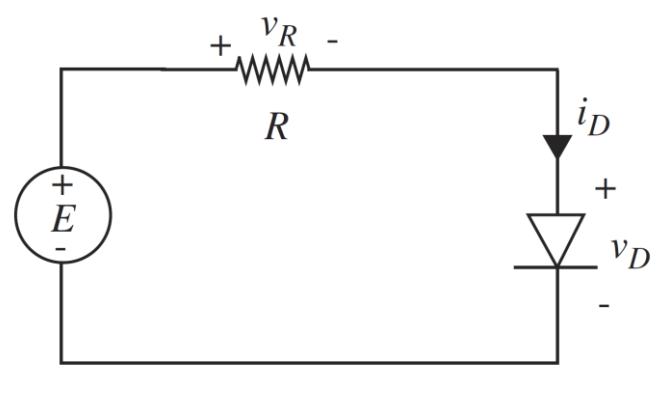
\includegraphics[width=0.5\textwidth]{images/circuit1.png}
		\end{figure}
	\end{problem}
	
	\begin{solution}
		1.
		\begin{table}[h]
			\begin{tabular}{| l | l | l | l | l | l | l | l | l | l | l | l |}
				\hline
				Try          & 1 & 2 & 3 & 4 & 5 & 6 & 7 & 8 & 9 & 10 & 11 \\ \hline
				R (\(\Omega\))   &   &   &   &   &   &   &   &   &   &    &    \\ \hline
				V$_{D}$ (V)  &   &   &   &   &   &   &   &   &   &    &    \\ \hline
				V$_{R}$ (V)  &   &   &   &   &   &   &   &   &   &    &    \\ \hline
				i$_{D}$ (mA) & 20 & 30 & 50 & 80 & 120 & 160 & 200 & 240 & 280 & 320 & 350 \\ \hline
			\end{tabular}
		\end{table}
		\newline
		2.
	\end{solution}
	
	\begin{problem}
		In this exercise, we would like to build a full wave rectifier using a diode bridge.
		\newline
		1. Construct the following circuit using:\\
		R\(_{L}\)=10K\(\Omega\)\\
		D is 1N4001\\
		V\(_{i}\)=20sin(100\(\pi\)t)\\
		\newline
		2. Measure the input voltage and current using a multimeter.
		\newline
		3. Measure the output voltage on R\(_{L}\) using a multimeter and an oscilloscope.
		\newline
		4. Compare the measurements with your calculations
		\newline
		5. (Optional) Use a 470\(\mu\)F capacitor in parallel with R\(_{L}\) and measure the output voltage.
		\begin{figure}[h!]
			\centering
			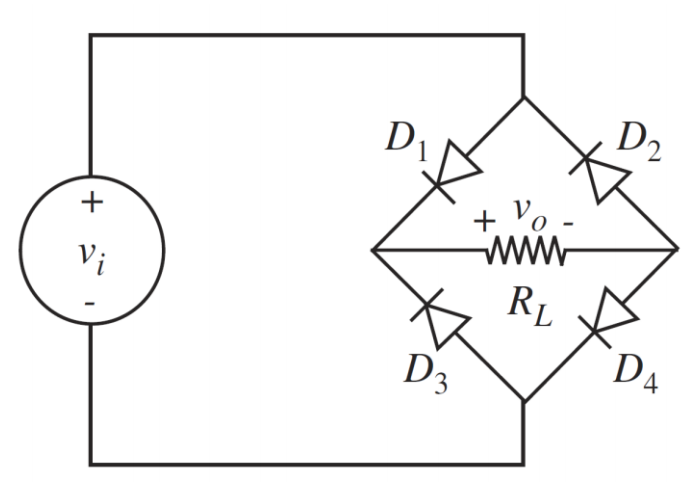
\includegraphics[width=0.5\textwidth]{images/circuit2.png}
		\end{figure}
	\end{problem}
	
	\begin{solution}
		1.
		\newline
		2.
		\newline
		3.
		\newline
		4.
		\newline
		5.
	\end{solution}
	
	\begin{problem}
		Using an OpAmp TL082, construct an inverting amplifier of gain 2.
		\newline
		V\(_{i}\)=1.5v\\
		V\(_{CC}\)=12v\\
		Output current should not exceed 10mA
		\newline
		1. Measure the output voltage and compare with your expectations.
		\newline
		2. Use V\(_{i}\)=2sin(100\(\mu\)t) and measure the output voltage using an oscilloscope.
		\begin{figure}[h!]
			\centering
			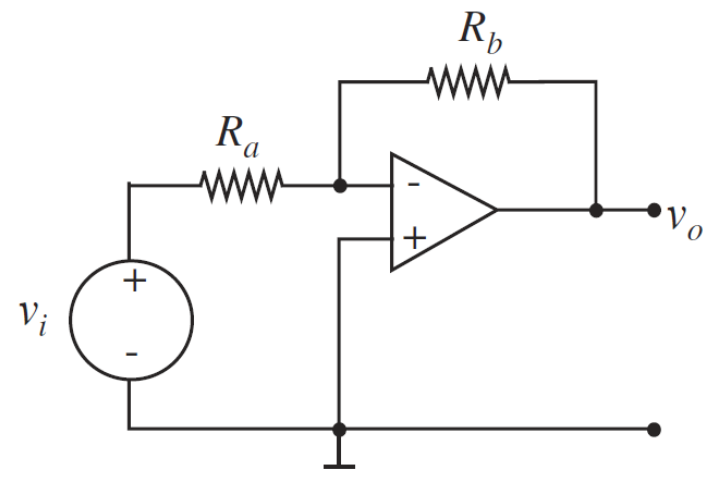
\includegraphics[width=0.5\textwidth]{images/circuit3.png}
		\end{figure}
	\end{problem}
	
	\begin{solution}
		1.
		\newline
		2.
	\end{solution}
	
	\pagebreak
	
	\large \bf{\textsc{\section{Lab 4}}
	\begin{problem}
		Using an OpAmp TL082, construct an amplifier that can deliver the following functions. Evaluate your circuit practically and theoretically.
		\newline
		1. z = 0.2x + y\\
		2. z = 3(x-y)\\
	\end{problem}
	
	\begin{solution}
		1. 
		\newline
		2.
	\end{solution}
	
	\begin{problem}
		We would like to investigate the properties of the MOSFET type BS170. Construct the following circuit with R=1K\(\Omega\). (a and b are equivalent)
		\begin{figure}[h!]
			\centering
			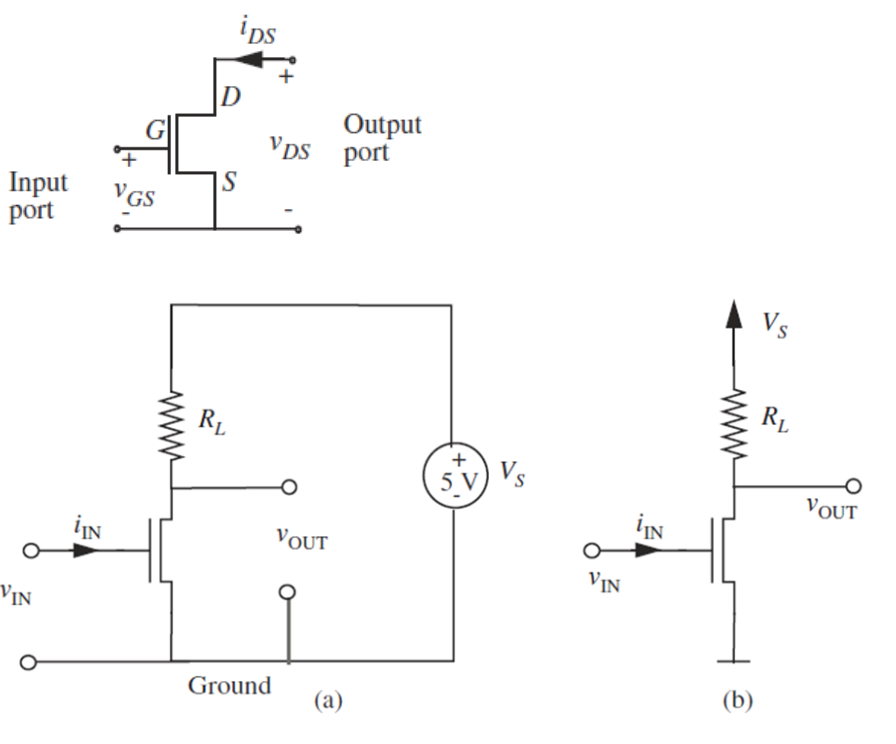
\includegraphics[width=0.5\textwidth]{images/circuit4.png}
		\end{figure}
		1. Measure the V\(_{out}\) and i\(_{DS}\) for the MOSFET for different values of V\(_{IN}\) and fill the table.
		\begin{table}[h]
			\begin{tabular}{| l | l | l | l | l | l | l | l | l | l | l | l |}
				\hline
				Try & 1 & 2 & 3 & 4 & 5 & 6 & 7 & 8 & 9 & 10 & 11 \\ \hline
				V$_{OUT}$ (V) & & & & & & & & & & & \\ \hline
				V$_{IN}$ (V) & 0 & 1 & 1.9 & 2.1 & 2.3 & 2.5 & 2.7 & 2.9 & 3 & 4 & 5 \\ \hline
			\end{tabular}
		\end{table}
		2. Plot your input-output characteristics of the MOSFET. What is the treshold voltage V\(_{T}\) for V\(_{GS}\)? Compare your findings with the datasheet.
		\newline
		3. Measure the V\(_{DS}\) and i\(_{DS}\) for the MOSFET for different values of V\(_{S}\) and fill the table \textbf{once the MOSFET is on}.
		\begin{table}[h]
			\begin{tabular}{| l | l | l | l | l | l | l | l | l | l | l | l |}
				\hline
				Try & 1 & 2 & 3 & 4 & 5 & 6 & 7 & 8 & 9 & 10 & 11 \\ \hline
				V$_{OUT}$ (V) & & & & & & & & & & & \\ \hline
				V$_{S}$ (V) & 5 & 6 & 7 & 8 & 9 & 10 & 11 & 12 & 13 & 14 & 15 \\ \hline
				i$_{DS}$ (mA) & & & & & & & & & & & \\ \hline
			\end{tabular}
		\end{table}
		4. Plot the I-V characteristics of the MOSFET and obtain R\(_{ON}\). Compare your findings with the datasheet.
	\end{problem}
	
	\begin{solution}
		1.
		\newline
		2.
		\newline
		3.
		\newline
		4.
	\end{solution}
	
	\begin{problem}
		Using MOSFET type BS170, construct circuits that represent the following logic functions. Evalute your circuit practically and theoretically.
		\newline
		1. A+B+C \\
		2. A.B+\(\overline{C}\) \\
		3. A.B+C \\
		4. \(\overline{A.\overline{B}+\overline{C}}\)
	\end{problem}
	
	\begin{solution}
		1.
		\newline
		2.
		\newline
		3.
		\newline
		4.
	\end{solution}
\end{document}

